% Options for packages loaded elsewhere
\PassOptionsToPackage{unicode}{hyperref}
\PassOptionsToPackage{hyphens}{url}
\documentclass[
]{article}
\usepackage{xcolor}
\usepackage{amsmath,amssymb}
\setcounter{secnumdepth}{-\maxdimen} % remove section numbering
\usepackage{iftex}
\ifPDFTeX
  \usepackage[T1]{fontenc}
  \usepackage[utf8]{inputenc}
  \usepackage{textcomp} % provide euro and other symbols
\else % if luatex or xetex
  \usepackage{unicode-math} % this also loads fontspec
  \defaultfontfeatures{Scale=MatchLowercase}
  \defaultfontfeatures[\rmfamily]{Ligatures=TeX,Scale=1}
\fi
\usepackage{lmodern}
\ifPDFTeX\else
  % xetex/luatex font selection
\fi
% Use upquote if available, for straight quotes in verbatim environments
\IfFileExists{upquote.sty}{\usepackage{upquote}}{}
\IfFileExists{microtype.sty}{% use microtype if available
  \usepackage[]{microtype}
  \UseMicrotypeSet[protrusion]{basicmath} % disable protrusion for tt fonts
}{}
\makeatletter
\@ifundefined{KOMAClassName}{% if non-KOMA class
  \IfFileExists{parskip.sty}{%
    \usepackage{parskip}
  }{% else
    \setlength{\parindent}{0pt}
    \setlength{\parskip}{6pt plus 2pt minus 1pt}}
}{% if KOMA class
  \KOMAoptions{parskip=half}}
\makeatother
\usepackage{graphicx}
\makeatletter
\newsavebox\pandoc@box
\newcommand*\pandocbounded[1]{% scales image to fit in text height/width
  \sbox\pandoc@box{#1}%
  \Gscale@div\@tempa{\textheight}{\dimexpr\ht\pandoc@box+\dp\pandoc@box\relax}%
  \Gscale@div\@tempb{\linewidth}{\wd\pandoc@box}%
  \ifdim\@tempb\p@<\@tempa\p@\let\@tempa\@tempb\fi% select the smaller of both
  \ifdim\@tempa\p@<\p@\scalebox{\@tempa}{\usebox\pandoc@box}%
  \else\usebox{\pandoc@box}%
  \fi%
}
% Set default figure placement to htbp
\def\fps@figure{htbp}
\makeatother
\ifLuaTeX
  \usepackage{luacolor}
  \usepackage[soul]{lua-ul}
\else
  \usepackage{soul}
\fi
% definitions for citeproc citations
\NewDocumentCommand\citeproctext{}{}
\NewDocumentCommand\citeproc{mm}{%
  \begingroup\def\citeproctext{#2}\cite{#1}\endgroup}
\makeatletter
 % allow citations to break across lines
 \let\@cite@ofmt\@firstofone
 % avoid brackets around text for \cite:
 \def\@biblabel#1{}
 \def\@cite#1#2{{#1\if@tempswa , #2\fi}}
\makeatother
\newlength{\cslhangindent}
\setlength{\cslhangindent}{1.5em}
\newlength{\csllabelwidth}
\setlength{\csllabelwidth}{3em}
\newenvironment{CSLReferences}[2] % #1 hanging-indent, #2 entry-spacing
 {\begin{list}{}{%
  \setlength{\itemindent}{0pt}
  \setlength{\leftmargin}{0pt}
  \setlength{\parsep}{0pt}
  % turn on hanging indent if param 1 is 1
  \ifodd #1
   \setlength{\leftmargin}{\cslhangindent}
   \setlength{\itemindent}{-1\cslhangindent}
  \fi
  % set entry spacing
  \setlength{\itemsep}{#2\baselineskip}}}
 {\end{list}}
\usepackage{calc}
\newcommand{\CSLBlock}[1]{\hfill\break\parbox[t]{\linewidth}{\strut\ignorespaces#1\strut}}
\newcommand{\CSLLeftMargin}[1]{\parbox[t]{\csllabelwidth}{\strut#1\strut}}
\newcommand{\CSLRightInline}[1]{\parbox[t]{\linewidth - \csllabelwidth}{\strut#1\strut}}
\newcommand{\CSLIndent}[1]{\hspace{\cslhangindent}#1}
\setlength{\emergencystretch}{3em} % prevent overfull lines
\providecommand{\tightlist}{%
  \setlength{\itemsep}{0pt}\setlength{\parskip}{0pt}}
\usepackage{bookmark}
\IfFileExists{xurl.sty}{\usepackage{xurl}}{} % add URL line breaks if available
\urlstyle{same}
\hypersetup{
  hidelinks,
  pdfcreator={LaTeX via pandoc}}

\author{}
\date{}

\begin{document}

\section{A Decent Proposal}\label{a-decent-proposal}

\emph{notes: \textasciitilde9000 words (without references)}

\subsection{Introduction}\label{introduction}

In this thesis, I will develop and experiment within an aesthetic of
`contemplative play,' a play with the potential to more clearly show the
nature of the world around us, and who we are within that world. The
functionality of play, the nimble maneuvering of people together within
a system, is a unique form of meaning-making that, in an age of
fractured attention and instrumentalized leisure, offers a compelling
alternative: a space of purposeless engagement where we encounter
ourselves, others, and the world afresh. Where many games try to guide
the player through specified challenges and defined narratives,
contemplative play points the player toward an openness that provides
the opportunity for introspection at a deeper, more ambiguous level. And
this new potential of playful contemplation offers an antidote to many
of the ways that people feel ill-at-ease with modern life.

Contemporary society has created a situation in which people feel
overwhelmed, with fractured attention and the pressure to be continually
active and productive. Many academics and artists have begun to push
back on the narrative that a life is just a series of quantifiable
achievements. Jenny O'Dell is a key voice in this movement, publishing
books such as \emph{How to do Nothing} \%\% cite \%\% and \emph{Saving
Time} \%\% cite \%\%, but many others have noted the pull to have a more
meaningful relationship with the world than what the design of our
technologies seems to dictate. We act and act, without giving ourselves
time to reflect, to contemplate the nature of the world. In the past,
art fulfilled this purpose. The paintings in our museums, the music in
our recital halls, and the stories in our literature would give us
opportunities for contemplation, but now even our leisure time is full
of activity and over-stimulation. Philosopher Byung-Chul Han laments
this loss of respite, saying ``\,`Leisure time' lacks both intensity of
life and contemplation. It is a time that we kill so as not to get
bored. It is not \emph{free, living time}; it is \emph{dead time}.''
(Han and Steuer 2023) \%\% {[} M: We'll see how this works {]} \%\% In
contrast, he claims ``we owe true happiness to the useless and
purposeless, to what is intentionally convoluted, what is unproductive,
indirect, exuberant, superfluous, to beautiful forms and gestures that
have no use and serve no purpose.'' \%\% cite \%\% He names this concept
``ceremonious inactivity'' where ``we do something, but to no end,'
resulting in the discovery of a reality that''reveals itself only to
contemplative attention.'' \%\% cite \%\%

Play is an ideal vehicle for this `ceremonious inactivity.' It is a
powerful and increasingly common way to engage with the world around us.
For decades, game designers and researchers have claimed that play
provides an opportunity to understand fundamental aspects of human
existence. Bernie De Koven, a foundational figure in this movement,
speaks to how play can elicit ``a shared transcendence of personal
limitations, of our understanding of our capabilities; a sudden,
momentary transformation of our awareness of the connections between
ourselves, each other, and the world we find each other in.'' \%\% cite
\%\% Similarly, in his book \emph{Play Matters}, Miguel Sicart states
that ``{[}t{]}o play is to be in the world. Playing is a form of
understanding what surrounds us and who we are, and a way of engaging
with others. Play is a mode of being human.'' \%\% cite \%\%
Designer/researcher Frank Lantz argues that the very nature of play as
being outside normal life contributes to its aesthetic value: ``It is
this distance that gives aesthetic experiences their power to be
\emph{about} life, its purpose and values.'' \%\% cite \%\%

This aesthetic understanding of play provides a helpful framework with
which to analyze the experience. In his book \emph{Design Aesthetics,}
Mads Nygaard Folkmann states that ``aesthetics gives way for a
reflection of how we perceive, sense, and are present in the world --
that is, how we relate to our surroundings.'' \%\% cite \%\% Common
understanding of aesthetics can be slippery, with definitions stretching
back to Plato and Kant and covering concepts such as phenomenology,
art-for-art's-sake, and epistemology. However, taking from Yuriko
Saito's concept of `everyday aesthetics', which encompasses ``the
sensuous and/or design qualities of any object, phenomenon, or
activity,'' \%\% cite \%\% we can better develop a functional scaffold
with which to approach the design and analysis of both play and
contemplative experience. Game designers and researchers have put a lot
of time and effort into developing a whole host of frameworks of the
foundational building blocks of games, but an aesthetic understanding of
play helps us to take a wider look. From this expanded perspective we
can look at particular lenses of aesthetic engagement and how they
contribute to the play as experienced by the player. With this expanded
scope, and leaning on an aesthetic structure that I often think about in
my own design practice, I propose looking at four distinct components of
play: Player(s), Playthings, Playgrounds, and Playtime. These aesthetic
pillars will give us helpful vantage points from which to think about
how play intersects with the contemplative mode.

Contemplative play offers a way of engagement that is both reflective
and participatory - an approach to dwell with and on the world and its
inhabitants in a playful manner. The aesthetic lenses of Players,
Playthings, Playgrounds, and Playtime will provide a framework to
analyze the various ways and environments that make play
`contemplative.' For each aesthetic pillar, I propose to read related
work and build out playful experiments in response to these ideas. In
addition, I will position this work in communication with other artistic
practices that encourage a contemplative engagement with the world along
similar aesthetic spheres---such as soundwalks, deep listening,
performative objects, contemplative architecture, and ambient media.
Through this reflective design practice - making playful experiments in
response to each of these aesthetic elements, reflecting on the nature
of play experienced through these explorations, and leveraging the
method for design materialization (MDM) for more profound insights - we
will gain more crystallized knowledge about that potential, and develop
ways to cultivate more engaging and meaningful play experiences.

\subsection{Background}\label{background}

\subsubsection{Reflective Design}\label{reflective-design}

In his 1982 book \emph{The Reflective Practitioner}, Donald Schön sets
up his argument for ``reflection-in-action,'' \%\% cite \%\% a way of
thinking about design practice that has been adopted by academics and
practitioners alike (Frayling, Redström, Eklund et. al, etc) \%\% cite
\%\%. Though this design process-focused understanding of ``reflective
practice'' is perhaps most commonly discussed with a focus on the
designers themselves, we can also think about how as designers we can
build ``reflective practices'' in to our designs. \%\% {[}P: Oh that's
quite nice. Did I miss this previously? Seems like an intriguing avenue
to follow, has anyone done this before?{]} \%\% \%\% {[}M: Not in games
maybe? But definitely if we look at Sengers, Performative Objects,
etc{]} \%\%

The concept of reflection has found a strong foothold in the academic
world, where it becomes a desired state for learners. Numerous thinkers
and educators have relied on Dewey's concept of `reflective thought' as
a goal for teaching. \%\% cite \%\% Dewey explains this state as
``active, persistent, and careful consideration of any belief or
supposed form of knowledge.'' \%\% cite \%\% Dewey and those who follow
focus on how reflection helps the learner learn. For them, the goal is
the gaining of knowledge. Jennifer Moon, for instance, states that
reflection is ``a mental process of thinking about what we have done,
learned, and experienced.'' \%\% cite \%\% This understanding of
reflection is unambiguous and practical, something to be harnessed for a
desired end outcome.

Similarly, in their paper ``Reflective Design,'' Phoebe Sengers et al.,
\%\% cite \%\% build on critical theory to argue for designs that brings
``unconscious aspects of experience to conscious awareness, thereby
making them available for conscious choice.'' \%\% cite \%\%
Specifically, they ``expand on reflection-in-action by not waiting for
surprise to occur but by intervening to create or stimulate these
reflection triggers.'' \%\% cite \%\% This shifts the focus of
reflection away from the nature of the designed object and instead
places it on the nature of technology as a whole. Sengers et al.~argue
that by focusing on the user's critical reflection, designers are able
to counter norms and create positive social effect.

However, there is also an opportunity for designing more ambiguous
reflective experiences. One possibility is through experimental
interactions. Lars Hallnäs and Johan Redström's \%\% cite \%\% ``Slow
Technology - Designing For Reflection'' introduces the concept of ``slow
technology {[}\ldots{]} as a tool for making reflection inherent in
design expression.'' \%\% cite \%\% They propose that slowing down,
removing clarity, and building friction into designs can make the user
reflect on the nature and role of technology in their life. A doorbell
that influences several fans behind an array of fabric squares
communicates something different from the usual chime, but what exactly?
The user is left to consider these objects and interactions and what
they might mean. This is similar to Rilla Khaled's proposal of a
`reflective game design,' where the designer designs to highlight
questions over answers, disruption over comfort, and reflection over
immersion. \%\% cite \%\% These types of games are designed in stark
contrast to serious games, which often have an underlying lesson to be
learned. Rather, reflective game design is a space where ``asking
meaningful questions is more important than providing clear answers.''
\%\% cite \%\% \#\#\# Contemplative Design

In order to differentiate the present work from the widespread use of
`reflective design' as a means for targeted critical reflection, I
propose the term \emph{contemplative design}. The word contemplation
stems from the latin \emph{com} + \emph{templum}, and was originally
``to mark out a space for observation.'' \%\% cite \%\% . From this
tradition, translators rendered the earlier Greek term~\emph{theōría},
used by both Plato and Aristotle, into the Latin~\emph{contemplatio},
which gets used in both the Platonic contemplation of eternal Forms and
the Aristotelian notion of contemplation as the highest form of human
happiness. \%\% cite \%\% Later, the term took on a more religious and
spiritual tone, especially popularized by the twentieth century Trappist
monk, Thomas Merton, and his book ``Seeds of Contemplation.'' \%\% cite
\%\% More recently, scholars such as Byung-Chul Han \%\% cite\%\% and
Oludamini Ogunnaike \%\% cite \%\%, have expanded the idea of
contemplation into a more mysterious interplay between humans and the
world. This use of `contemplation' gets more to the root of what a deep
interaction with designed experiences could feel like. In their paper
``Contemplative Neuroaesthetics and Architecture: A Sensorimotor
Exploration,'' Djebbara et al.~\%\% cite \%\% use the term to indicate
``heightened level of awareness and an intentional focus on the present
moment, fostering a state of deep reflection and non-judgmental
engagement.'' \%\% cite \%\% Using examples from architecture, including
the Rundetårn in Copenhagen, Denmark, Louis Kahn's Salk Institue in La
Jolla, California, and the Chartres Cathedral in France, Djebbara et
al.~argue that these buildings can bring about states of deep
contemplation/reflection in a viewer by ``enforcing an embodied
experience of presence. \%\% cite \%\% Indeed an entire field of
contemplative architecture has developed that explores how architectural
spaces of all kinds can foster these kinds of deeper experiences. \%\%
cite \%\%

We see this focus on contemplative design in other places as well. Such
designs are often art objects, with critical design and speculative
design as example approaches. Anthony Dunne's Faraday Chair, for
example, uses a large Faraday cage to create a haven from
electromagnetic fields, which causes the viewer to ask, ``If the inside
is empty, what is outside?'' \%\% cite \%\% Additionally, the ``chair''
is actually a daybed, which Faraday claims contributes to the notion
that ``once electromagnetic fields are taken into consideration,
conventional assumptions about everyday objects need to be reexamined.''
\%\% cite \%\%. In Critical Play, Mary Flanagan calls these the designs
that ``represent one or more questions about aspects of human life.''
\%\% cite \%\% This `critical play' is a type of play that pokes at the
very nature of play itself (rules, competition, playspaces, for example)
and uses that questioning stance to reflect on the world at large.

Soundwalking is another field of artistic practice related to my
understanding of contemplative design. Soundwalking started as part of
R. Murray Schafer's \emph{World Soundscape Project}, \%\% cite \%\%
which arose from active listening practices developed by artists like
John Cage and Pauline Oliveros. \%\% cite \%\% Schafer and those in the
project sought to anchor these active listening practices to a given
place. Hildegard Westerkamp especially believed that through
soundwalking, listeners could better understand their sonic
environments. \%\% cite \%\%

Janet Cardiff and George Bures Miller use their recorded soundwalks to
guide the listener through a world of their making, a sonic world that
is overlaid onto a real, physical place. \%\% cite \%\% In \emph{Her
Long Black Hair}, as the listener walk through Central Park in New York
City, snippets of conversation slip by that feel like they are in the
same space as you. Cardiff speaks directly to you but then has a
conversation with others who are not visibly present. Recorded audio
effects of long-gone marching bands, sirens, and political rallies make
the listener feel like they are experiencing a highly professional radio
drama, creating a space for deep and truly unique contemplative
experiences where ``our seemingly dull everyday existence has the
potential to reveal simultaneous magical worlds of experience.'' \%\%
cite \%\% (24) \%\% {[} P: Might you get push-back on whether or why
this leads to contemplation? Currently this is more an assertion\ldots{}
{]} \%\% \%\% {[}M: Maybe? I sure felt very contemplative at certain
points{]} \%\%

Kristina Niedderer's ``performative objects'' are another noteworthy
example. \%\% cite \%\% She distinguishes these objects from Jacques
Carelman's \emph{Catalogue d'Objets Introuvables} \%\% cite \%\% by
describing them as, ``objects that can cause mindfulness in the context
of everyday use, and not in the institutional context of art.'' \%\%
cite \%\% This separation means that the performative object must rely
on adaptations within its formal elements to create a contemplative
state \emph{while remaining functional.} This is particularly
interesting as we consider designing contemplative experiences for
game-like experiments that retain their sense of play. \%\% {[} P: I
like the thing here of specifically identifying something you'll want to
return to, worth keeping an eye out for which other theorists contribute
something like this and consider whether it ought to be highlighted
further structurally {]} \%\%

Another reference point for contemplative design is ``ambient
interactive experiences.'' \%\% cite \%\% These designs build on ideas
from other slow, ambient media such as the music of Brian Eno \%\%
e.g.~\%\% and the films of Godfrey Reggio \%\% e.g.~\%\% to create a
more passive yet potentially deeper experience. The field of slow games
is a compelling and clear precedent for this, but thinking about ambient
media opens up the opportunity to include a lot more material. These
projects are interested in slow pacing, obfuscation, and less
``comfortable'' experiences, with varying degrees of success. Game
designer and researcher Tracy Fullerton refers to this as `reflective
play' where slowness isn't ``equivalent to meaningfulness, but rather
because the process of making meaning through reflection requires time
at a human pace, takes cycles of response, interpretation, and unpacking
of experience.'' \%\% cite \%\% Examples include the cooperative game
\emph{Journey} \%\% cite \%\%, the work of David O'Reilly \%\% cite \%\%
and Pippin Barr's \emph{v r 5} \%\% cite \%\%, among others. \#\#\#
Design Aesthetics

There are various existing frameworks for thinking about the elements of
play that might be relevant for a study of contemplation. While these
frameworks are often overly descriptive, there are elements withing that
can inform our current study, providing a solid foundation for our
exploration.

Salen and Zimmerman, in their book Rules of Play \%\% cite \%\%, set up
an understanding of meaningful play. In their definition, this relates
more to how the playful systems in a game relate meaning back to the
game itself. However, this could be expanded to how play could broaden
our understanding of meaning-making in the world. In A Game Design
Vocabulary \%\% cite \%\%, Anna Anthropy and Naomi Clark call this the
context of a game, discussing specifically how the design aspects of a
digital game (camera, character, sound, etc) communicate aspects of the
game to the player. Could we leverage the contexts of play, pointing
outward to contemplate on life in general? What are the specific
contexts that we could use to do so?

In \emph{The Art of Game Design: A Book of Lenses} \%\% cite \%\%, Jesse
Schell introduces the concept of lenses that we can use to develop and
evaluate games from specific vantage points. While it may be overkill to
apply each of his 113 lenses to our study, applying this concept of
lenses as a way to establish and evaluate context is a valuable
exercise. Hunicke et al.'s ``MDA: A Formal Approach to Game Design and
Game Research'' identifies three key components for game design:
Mechanics, Dynamics, and Aesthetics. Their concept of \emph{aesthetics}
as ``the desirable emotional responses evoked in the player, when she
interacts with the game system'' \%\% cite \%\% is a good starting
place, but is a slightly different understanding from mainstream design
aesthetics, where as Folkmann explains, at a broader level it ``offers
concepts for investigating and understanding how design is constituted,
how it appeals to and affects people, and how it frames human
experiencing.'' \%\% cite \%\%

Thinking of the context of play, specifically through these wider lenses
of design aesthetics, is an excellent framework with which to explore
how play could engender contemplative experience. \#\#\# Aesthetics of
Contemplative Play

Book III of Schopenhauer's \%\% cite \%\% ``The World as Will and
Representation'' holds some key language about what he calls ``aesthetic
contemplation,'' which is pertinent to the ideas of contemplation in
artistic fields. In section 34, he describes the shift from looking at
something through `reason' to ``a steady contemplation'' by saying:

\begin{quote}
if, instead of all this, we devote the entire power of our mind to
intuition and immerse ourselves in this entirely, letting the whole of
consciousness be filled with peaceful contemplation of the natural
object that is directly present, a landscape, a tree, a cliff, a
building, or whatever it might be, and, according to a suggestive figure
of speech, we \emph{lose} ourselves in this object completely, i.e we
forget our individuality, our will, and continue to exist only as pure
subject, the clear mirror of the object
\end{quote}

\%\% cite \%\%

This concept of aesthetic contemplation helps to specify the type of
aesthetic play experience that one could have, an experience that moves
from the surface to something deeper. What is especially helpful is how
Schopenhauer includes space for \emph{active} contemplation on the
viewer's part. It is not a passive, peaceful, zen calm, but rather an
attitude of looking that is searching for more. Some philosophers and
art historians have coined the term
\href{https://iep.utm.edu/aesthetic-attitude/}{``aesthetic attitude''}
to explain this idea. \%\% cite \%\%.

Combining this with an \emph{aesthetics of play}, we can create a series
of lenses with which to explore the idea of contemplation. I find that
Katja Kwastek's \%\% cite \%\% \emph{Aesthetics of Interaction in
Digital Art} is foundational here (and even includes a chapter on the
``Aesthetics of Play''). In my personal practice, I often think of four
big picture aspects of play. First, the players are those who willingly
engage with the playful systems. Second, the playthings are the
trappings of games, the objects with which the player interacts. Third,
the playspace is the boundary created by play, a boundary that is often
as much mental as physical. Lastly, playtime is the time set aside and
made `sacred' by the play, a time that expands and contracts to contain
more than the sum of its seconds. These four aesthetic lenses, when used
as a way to reflect on play, will give us a way to in to the discussion,
a way towards the construction of unique experiences with contemplation
in and through play.

\subsection{Methodology}\label{methodology}

This research relies on game experiments to examine the possibilities in
manipulating playful aesthetics towards contemplative ends. These
playful experiments will be tangible outputs to explore ideas found in
the overlap between playful aesthetics and contemplative design, with
knowledge arising both from the active building of these experiments as
well as in conversation with other designers. Each of these prototypes
will go through a series of stages. The overall trajectory for this
exploration will resemble the classic design process, with stages of
divergence and convergence throughout. As in the traditional interactive
design process, each stage of the process is evaluated in stasis by me
and in conversation with design peers. These conversations will lead to
new insights and feed into future iterations of the overall concepts.
\%\% {[} P: Hmm. It's quite stiff. I'll think further. {]} \%\%

Throughout this exploration, I will initially use an internal iterative
design process as a basis from which to pursue and evaluate my designs.
This is in alignment with ideas stemming from traditional iterative
design practice where designers rapidly develop and test many ideas on
an individual level, discarding anything that obviously doesn't work,
and refining all of the ideas down to a few testable prototypes. \%\%
Iterate? \%\% This method also relies on the design through research
practices as proposed by Frayling and Redström, in which knowledge is
gained through the practice of design. \%\% cite \%\%

Additionally, I will gain knowledge about my solution through
observation and conversations with other designers. Sharing work with
other designers who have deep experience in a discipline is a great way
to catch these early mistaken assumptions that I might be making about
my audience, goals, and proposed solutions. \%\% {[}P: Probably needs to
be deeper and more grounded to sound like it properly belongs in a PhD,
which I believe it does.{]} \%\%

\subsubsection{Foundations: Research Through Design, Design Practice,
and Practice-Based
Research}\label{foundations-research-through-design-design-practice-and-practice-based-research}

In his paper for the first issue of Research in Art and Design,
Christopher Frayling introduced his ideas for the relationship between
research and design. \%\% cite \%\% He distinguished between research
into art and design (where the research is historical, cultural or
theoretical), research through art and design (where the research is
into the processes and tools for future design methodologies), and
research for art and design (where the end product is an artifact). In
the years following, many researchers adapted these ideas, and the area
that Frayling labeled as research for art and design has become more
widely understood as research through design.

In their introduction to Perspectives on Design Research, Bærenholdt et
al.~\%\% cite \%\% refer to this mode as both research through design
and design-based research (including design through research) noting
that, ``design becomes as much a medium and process of research, as a
result.'' \%\% cite \%\% It is through the making of designs that
knowledge is gained, but how we exactly understand this relationship can
be more complex.

The specific framework that I employ to understand how my research and
designs are in conversation is firmly situated in Johann Redström's
tactic of Sequencing.\%\% cite \%\% Redström expands on Frayling's
concept of research through design and explores explicit tactics for how
these methods are employed. His concept of sequencing, where design and
theories are meant to coexist throughout the process, is of particular
interest. ``Using a highly iterative process, more developed relations
between theory and design can evolve as the understanding of how the
different design variables will have an impact on the test situation
grows deeper.'' \%\% cite \%\%

\st{I believe that t} The iterative design process is uniquely suited
and positioned to benefit from this concept of sequencing. As a
designer, it is fundamental that you document and reflect on your
designs and how they are being perceived by a given audience. In this
way, you are in constant conversation with the design, testing its
validity, and gaining knowledge in the process. \%\% {[}P: Very Schön-y
too{]} \%\%

This understanding of the benefits of the design process is echoed in
the concepts of practice-based research. Linda Candy, in the Routledge
International Handbook of Practice-Based Research, defines
practice-based research as ``a principled approach to research by means
of practice, in which the research and the practice operate as
interdependent and complementary processes leading to new and original
forms of knowledge.'' \%\% cite \%\% An important concept here is that
it is through the creations of these designed artifacts that the
researcher is able to test and gain knowledge about the world.

\subsubsection{Internal Iterative Game Design Process with the Method
for Design
Materialization}\label{internal-iterative-game-design-process-with-the-method-for-design-materialization}

The initial stages for this research will rely on my practice as a game
and sound designer. It is here where the most radical idea generation,
prototyping, reflection, and refinement will happen.

In \emph{The Reflective Practitioner}, Donald Schön argues that
``research is an activity of practitioners. It is triggered by features
of the practice situation, undertaken on the spot, and immediately
linked to action.'' \%\% cite \%\% I have found that this very
accurately describes my own game design process. As a designer, I am in
a dialog with my design, and the process involves thousands of decisions
that are repeatedly implemented and evaluated, with this interchange
happening throughout the entirety of the process.

In my practice, this process starts with a sketching phase. \%\% cite
Buxton? \%\% Ideas about visual style, game mechanics, themes, etc are
explored by rapidly sketching and reflecting on their feasibility and
design potential. The goal of this stage is to generate as many ideas as
possible, helping me think through the problem and generate possible
solutions. These ideas are then refined down to something more concrete
and actionable that I intend to build and test in the digital space. The
collateral from these sessions are captured using a camera to be
included in any online documentation.

Once the design process moves into the digital space, I use the game
engine Unity, image creation software Photoshop, and digital audio
workstations (DAWs) like Reaper and Ableton Live in conjunction to build
prototypes that implement some of the most promising ideas from the
ideation phase. As these prototypes are built, new ideas emerge and
those that do not work as intended are discarded. \%\% Maybe explicitly
point out the conversation with materials taking place here \%\% This
refinement happens repeatedly and at a very quick pace. Then, once the
ideas are more solidly understood, the process of refinement introduces
even quicker but far less radical incremental changes. This stage
adheres to Jesse Schell's Rule of the Loop, where ``the more times you
test and improve your design, the better your game will be.'' \%\% cite
\%\%

Through all of these phases, I implement the Method for Design
Materialization (MDM) first presented by Rilla Khaled, Jonathan Lessard,
and Pippin Barr \%\% cite \%\% in ``Documenting Trajectories in Design
Space: a Methodology for Applied Game Design Research.'' In this method,
the small decisions that a designer makes during the course of their
process are documented using the version control system Git \%\% {[} P:
GitHub is just the cloud storage platform in the end really {]} \%\%.
Any time that the designer uploads a commit, they write a detailed
message commenting on the particular design decision, motivations,
thoughts, and any future plans at that specific moment in time \%\% {[}
P: And sticking with Schön, reflections of conversations with material,
relationship to technical practice to design {]} \%\%. This then becomes
part of the overall archiving not only of a design's trajectory, but
also the designer's unique thought process. Khaled et al.~\%\% cite \%\%
state that the ``history of commits over time can give an understanding
of the overall design space and how it has been traversed: its pressure
points, its branching points, where decisions have been made, and where
possible lines of inquiry have been pruned.'' \%\% cite \%\% The most
important thing about this is that the large amount of qualitative data
produced makes it possible to use methods of analysis derived from
grounded theory \%\% {[} P: and thematic analysis, and CITE {]} \%\% to
organize, analyze, and develop theories about the information that is
generated. From this analysis, patterns can emerge to aid in reflection
on the solutions and suggest new possible directions for exploration.
\%\% {[} P: Going to want to expand on the analysis component here and
get explicit about the procedures. {]} \%\%

The end goal of all of this should be a playable prototype that has made
it through several phases of internal testing and refinement and is
ready to be shown to others. \%\% {[}P: Really, though, as per the
above, the end goal is a prototype \emph{and the archive of design
documentation}{]} \%\% Generally, I rely on my network of trusted
colleagues and friends for feedback on the work that I am making. These
are other game and/or sound designers and those whose opinion I can rely
on to give me valuable feedback. This sharing of work often sparks a
dialogue that helps me refine both the thing that I am making as well as
the entire thought around the conceptual side of the work. \%\% {[}P:
Should probably think of a way to formalize this a teeny bit, there's
probably some official methodological approach that describes this{]}
\%\%

This entire phase of the process will take place within the framework of
the MDM. All feedback will be documented and added to the project
repository \%\% {[}P: Think this is the first mention of a repository?
Need to check in on technical language and make sure it's always glossed
on first use{]} \%\%. This way it can be included in the overall
analysis of the design research. This synthesized information will then
be applied to further iterations on both this particular design solution
and future explorations. \%\% {[}P: I think you're saying that even the
analysis process is in the repo? May needed to be clearer{]} \%\%

\subsubsection{Summary}\label{summary}

In summary, my methodology for each iteration of this research will go
through a series of phases. Firstly through rapid prototyping on an
individual level, where my intuition \%\% {[}P: And experience
and\ldots{} probably want to sell yourself as experienced and already
good at this{]} \%\% as a designer will help to refine an initially
large amount of ideas to only those with the most potential. This design
through research practice will facilitate knowledge creation both about
==the problem and these possible solutions== \%\% {[}P: Bit vague{]}
\%\%. Additionally, I will leverage observations and conversations with
other designers to test these designs, quickly implementing what is
learned into a series of final playable prototypes that will arise from
the study that I am undertaking in each of these aesthetic lenses.
During the entirety of the design process, I will be using the method
for design materialization to document, track, and analyze both my
individual designs and the overall process to see what new knowledge can
be gained and what new solutions might arise.

\subsection{Timetable}\label{timetable}

In general, I propose to focus on each of the four main aesthetic-topic
areas for a set duration. During this focused time, I will read
literature and experience first-hand the art and design experiences in
this domain, responding to the material both in writing/reflecting and
creating playful exploration prototypes. Once the initial stages have
been complete, I will spend the remaining time on the synthesis and
writing of the thesis paper.

\begin{itemize}
\tightlist
\item
  Explorations

  \begin{itemize}
  \tightlist
  \item
    Player (Sep.~2025 - Dec.~2025)
  \item
    Playthings (Jan.~2026 - April 2026)
  \item
    Playgrounds (May 2026 - August 2026)
  \item
    Playtime (Sep.~2026 - Dec.~2026)
  \item
    Synthesis, Thesis Writing, and Revisions (Jan.~2027 - Dec.~2027)
    \%\% {[}P: Yep, fine by me. It's potentially the case you don't need
    the full year at the end, but why not right, and it's strategic at
    some level anyway, so all good.{]} \%\% \#\# Chapter Breakdown
  \end{itemize}
\end{itemize}

My initial idea here is to have each of the main chapters focus on an
aesthetic of contemplative play. Through each of these lenses, I will
look at a specific artistic practice from outside the realm of games and
then apply the lessons learned to a designed play experience. \%\% {[}P:
Feels like this can obviously be more confident and together. Not clear
you need a Part 1 and a Part 2, I think it can just be a series of
chapters{]} \%\%

\subsubsection{Part 1}\label{part-1}

\begin{verbatim}
- Introduction
- Background
- Methodology
\end{verbatim}

\%\% {[}P: The boring standard approach would just be Introduction,
Background, Method; if you want to go down that road.{]} \%\% \#\#\#
Part 2: Aesthetics in Contemplative Play

\%\% {[}P: It's not impossible you could be pinged a bit for these bits
being a little on the short end. Feels like you probably already have so
much more to say and project about the area + the project(s) you want to
talk about.{]} \%\% \#\#\#\# Player

In this chapter I will:

It will include the following sections:

Aesthetic description Related genre description Existing crossover Ideas
to explore

Much of play is performative. A player acts out scenarios. They move
their body in a coordinated effort with other players or the playful
system. Play can even be designed so that the act of playing is engaging
from those outside of the playspace. Professional sports is a clear
example of this, but Let's Plays, E-Sports, and arcade experiences (kids
gathered around a Street Fighter cabinet in the 90s or DDR machines in
the early aughts) also point to the possibilities of ``performing''
play.

Soundwalking is an excellent genre precedent to think about how not only
our physical bodies inhabit an experience, but also how the physical
world around us allows for performance. Artists like Hildegard
Westerkamp built on the active listening practices of Pauline Oliveros
and John Cage to invite listeners to playfully explore acoustic space.
Tapping on bridges, shouting in tunnels, banging on cans: these playful
acts require the listener to become performer in order to discover
something new about the world around them.

Thinking about the player as performer and how soundwalks (and other
interactive artworks) have used the movement of participants to create
meaning, what new contemplative and playful experiences can we create?

\begin{figure}
\centering
\pandocbounded{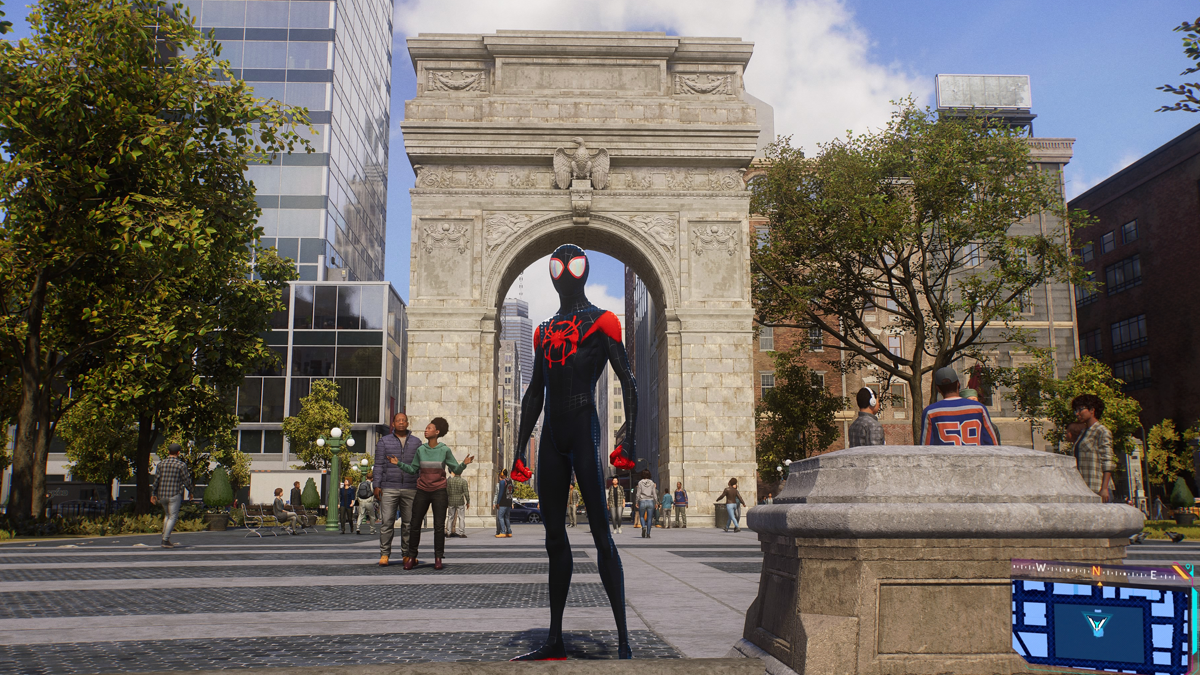
\includegraphics[keepaspectratio,alt={Miles Morales}]{../Media/spiderman.png}}
\caption{Miles Morales}
\end{figure}

Games and Soundwalks both operate in this area of ``performance,'' but
come from at it at slightly different angles. The game ``performance''
is generally much more about how the avatar ``performs'' that the actual
player. An early attempt to interweave soundwalks with play was a series
of soundwalks for the PS5 game \emph{Spiderman 2}, and while compelling
for a variety of reasons, this concept of performance remains
unexplored. \%\% cite the paper \%\%

\begin{figure}
\centering
\pandocbounded{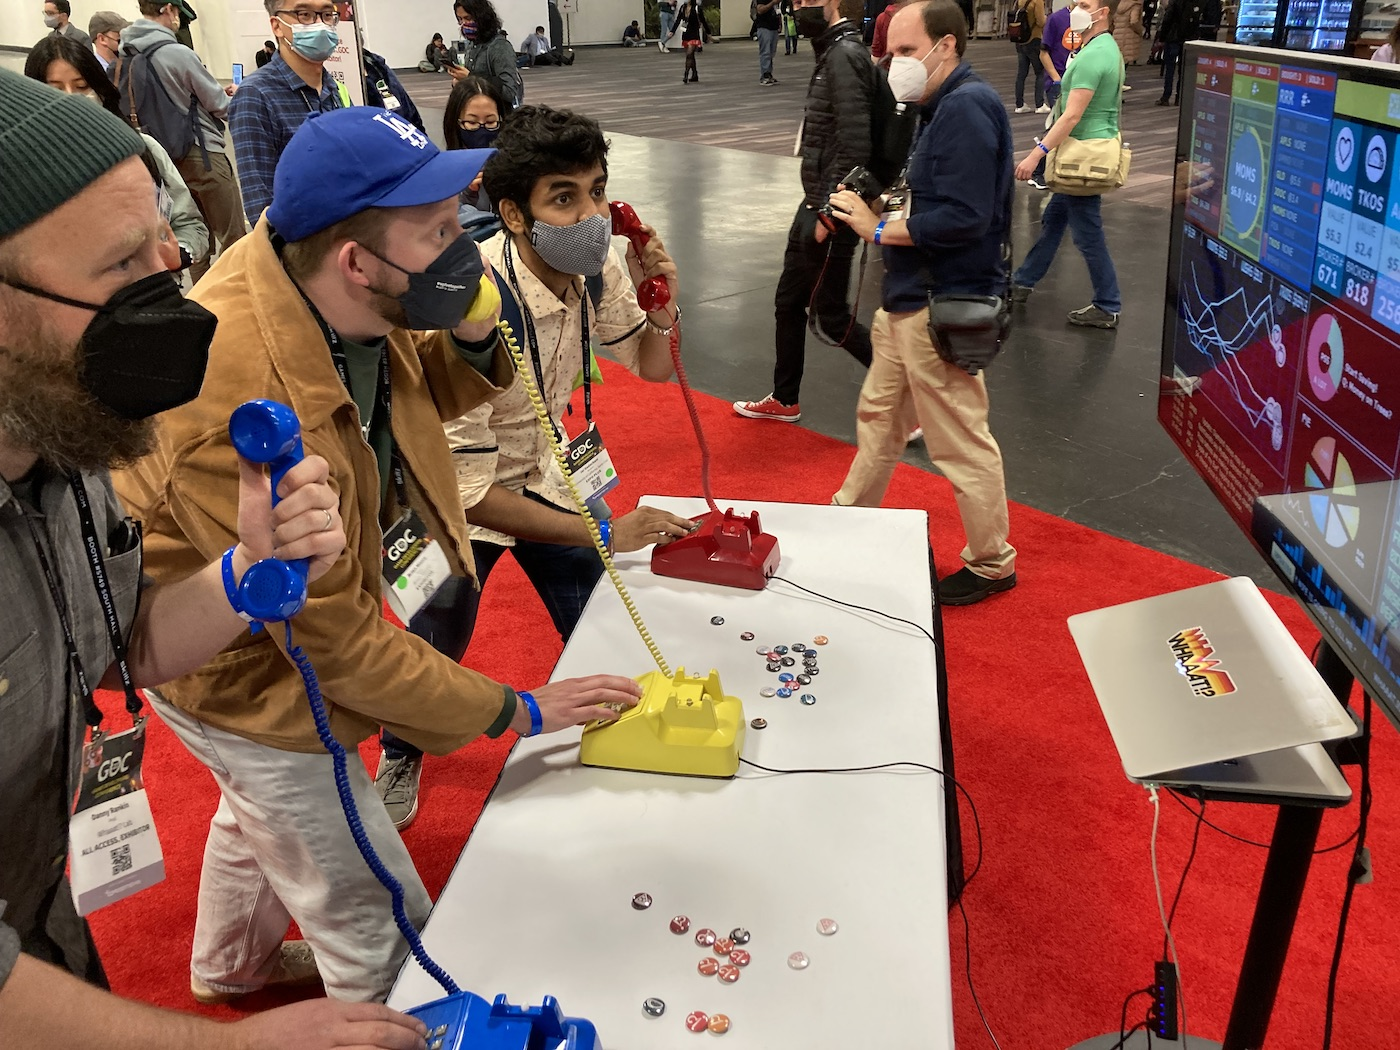
\includegraphics[keepaspectratio,alt={Buy! Sell!}]{../Media/bs.jpg}}
\caption{Buy! Sell!}
\end{figure}

Installation-based play, Like Buy! Sell! thinks about the player as
performer. In a similar way, playful soundwalks could be a space to
explore the overlap between play and performative spaces. Janet Cardiff
hints at these playful moments in her soundwalks, and future work (such
as the ``An Invitation to Play'' soundwalk accepted to ICMC 2025 in
Boston) will be a further exploration of these ideas.

\paragraph{Playspace}\label{playspace}

Space is a core aesthetic to the play experience. The concept of the
magic circle in particular, sets to explain the physical, and mental
demarcation between ``the real'' world and the imaginatively playful
world. It is this established structure that gives the player agency to
engage in playful acts, choosing one possible action over another and
reflecting on how those actions contribute to the imagined world.

Contemplative Architecture is similar in that the creation and
consecration of a space can engender different perspectives than the
ones a person came in with. Changes in sound, light, and material imbue
the space with a meaning in contrast to the outside world. Huizinga's
discussion of the ``play-festival-rite'' is of particular interest here,
as it provides a direct link between play and contemplative (even
sacred) spaces.

Focusing on this concept of the space in which play happens (i.e the
magic circle) and examples from Contemplative Architecture, how can we
create playfully contemplative experiences? Busy Work and TIKATMOS are
two games that explore this question by creating distinct (and physical)
gameworlds to facilitate a certain level of engaged play.

\begin{figure}
\centering
\pandocbounded{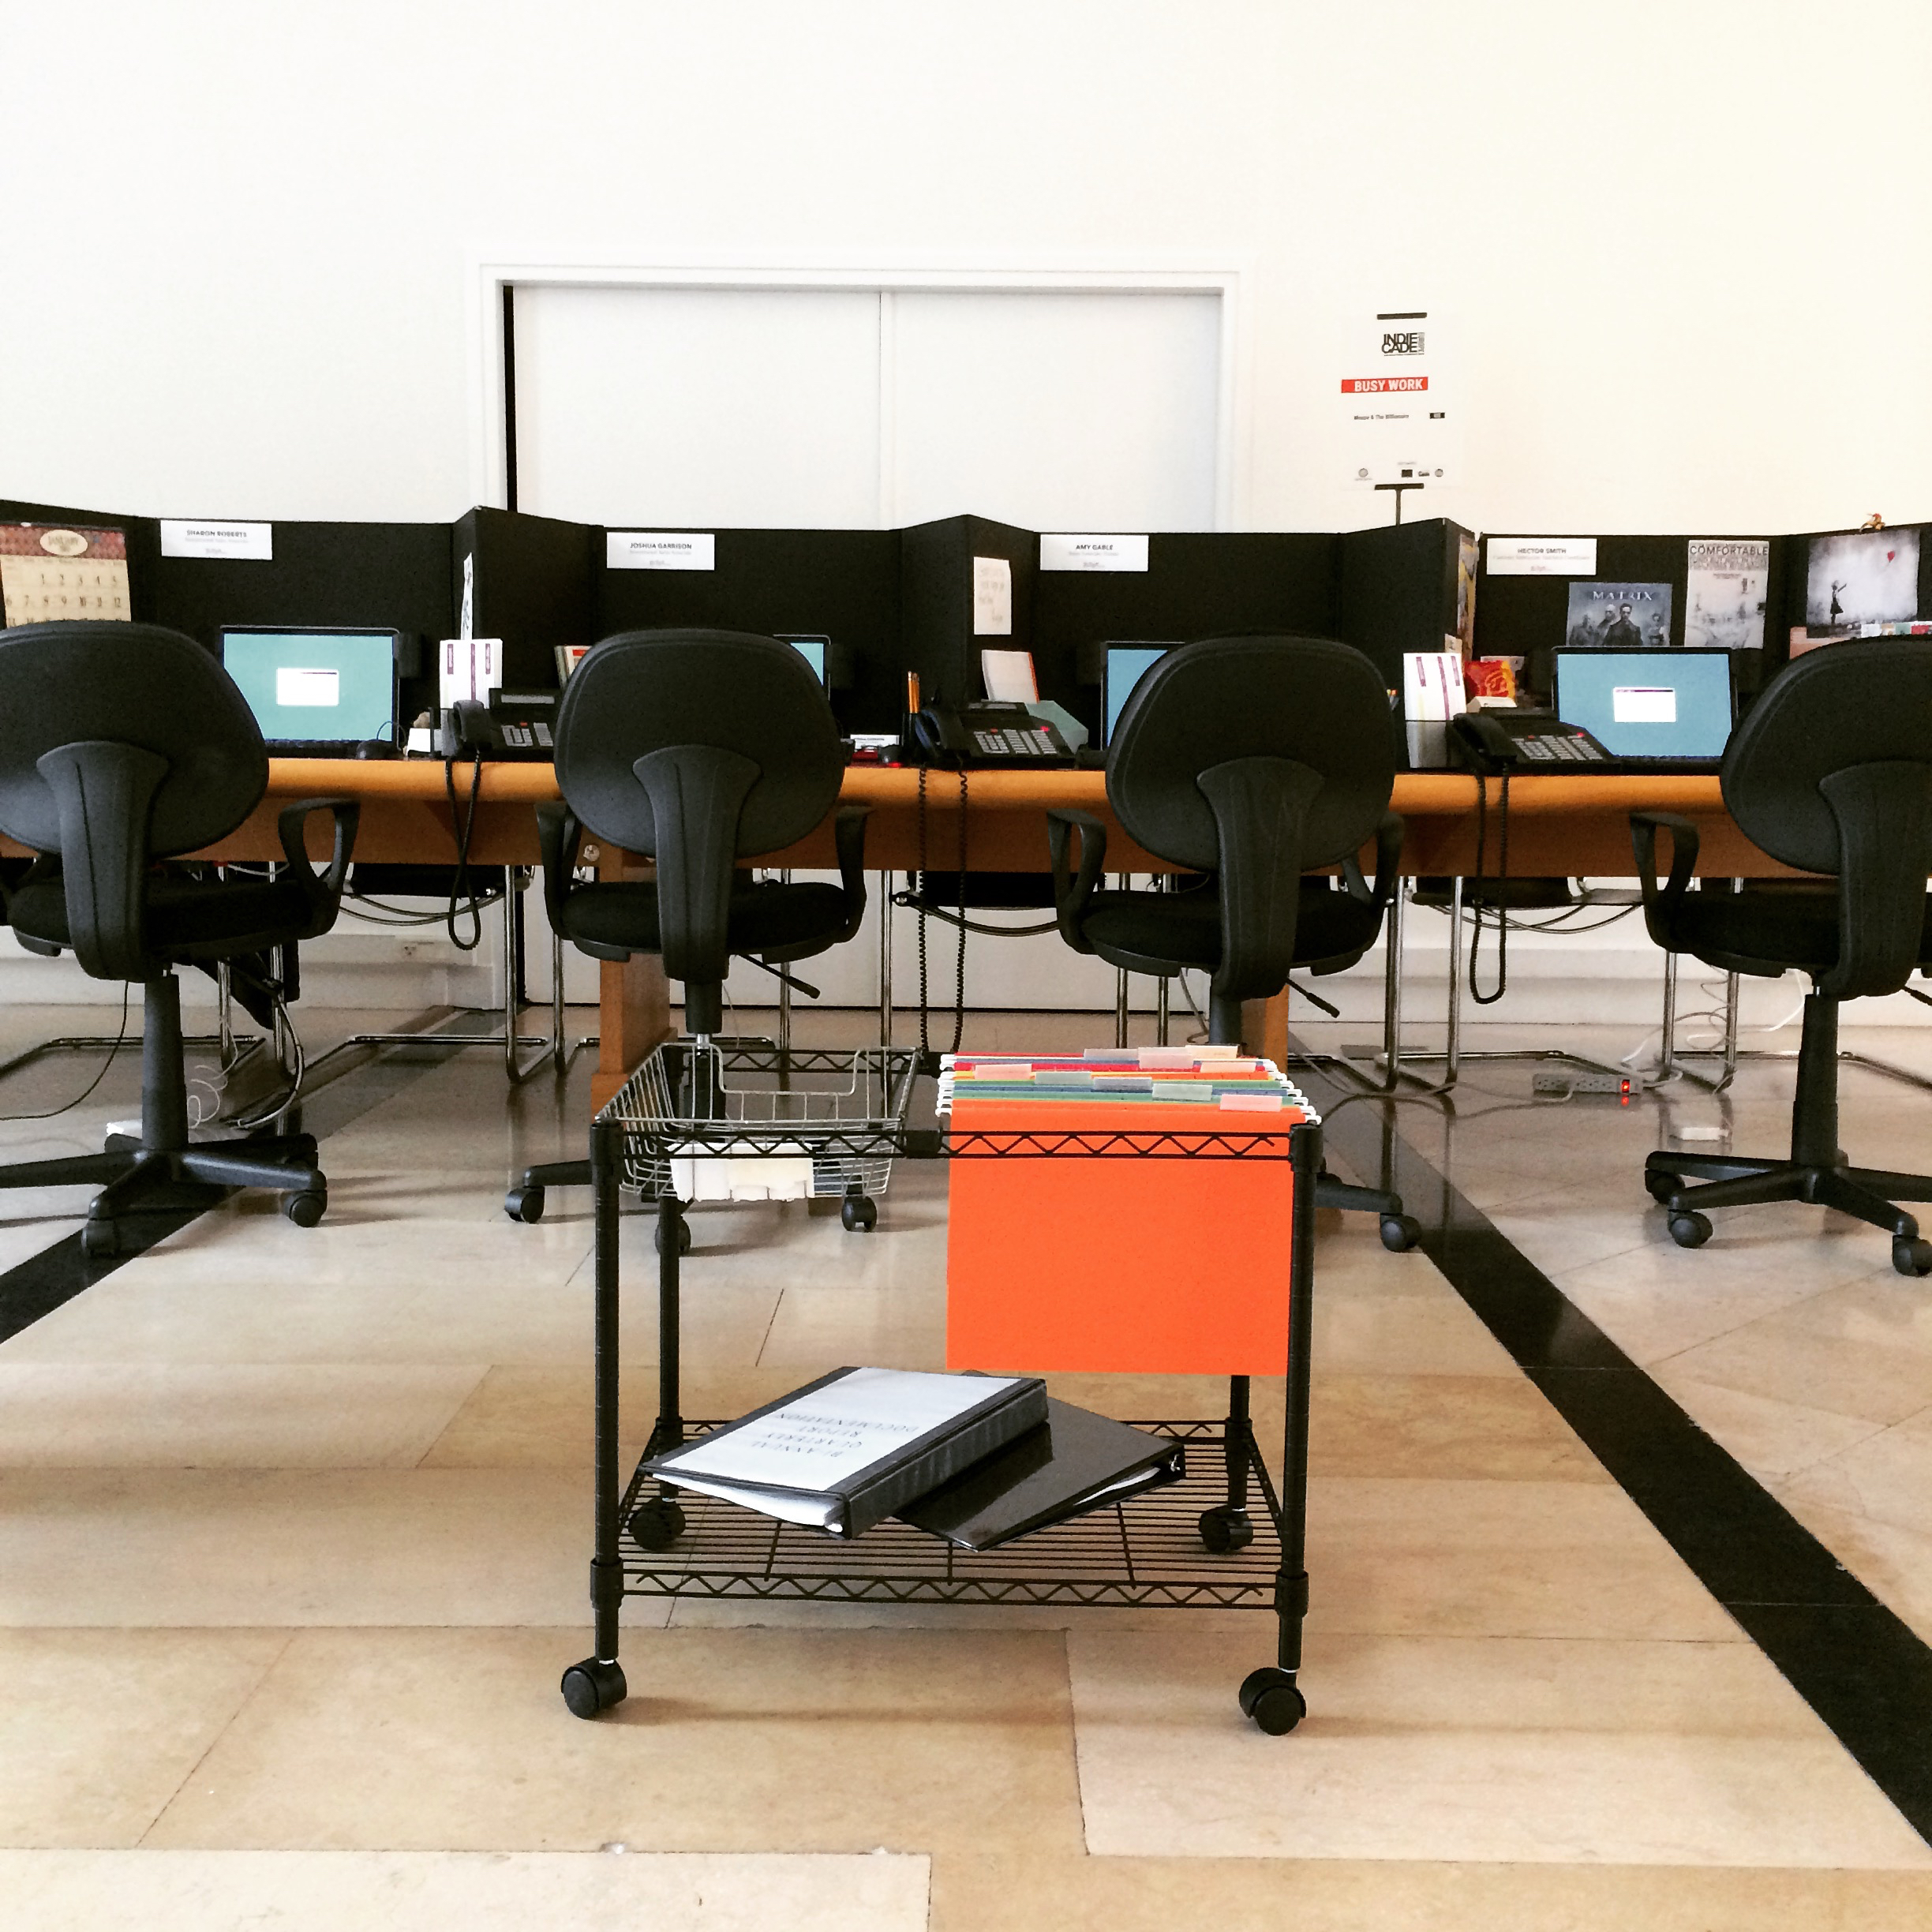
\includegraphics[keepaspectratio,alt={Busy Work}]{../Media/bw.jpg}}
\caption{Busy Work}
\end{figure}

Using narrative elements, physical actions, and environmental
storytelling through the built environment, Busy Work examines the
modern challenge of accomplishing work while juggling conflicting
priorities. Players are left wondering if what they do matters, whether
or not they are set up to fail and if the rewards are worth the effort.
People handle the mundane and possibly futile aspects of life in many
ways, and this work helps player to reflect on this by giving them
playful options based on lived experience.

\begin{figure}
\centering
\pandocbounded{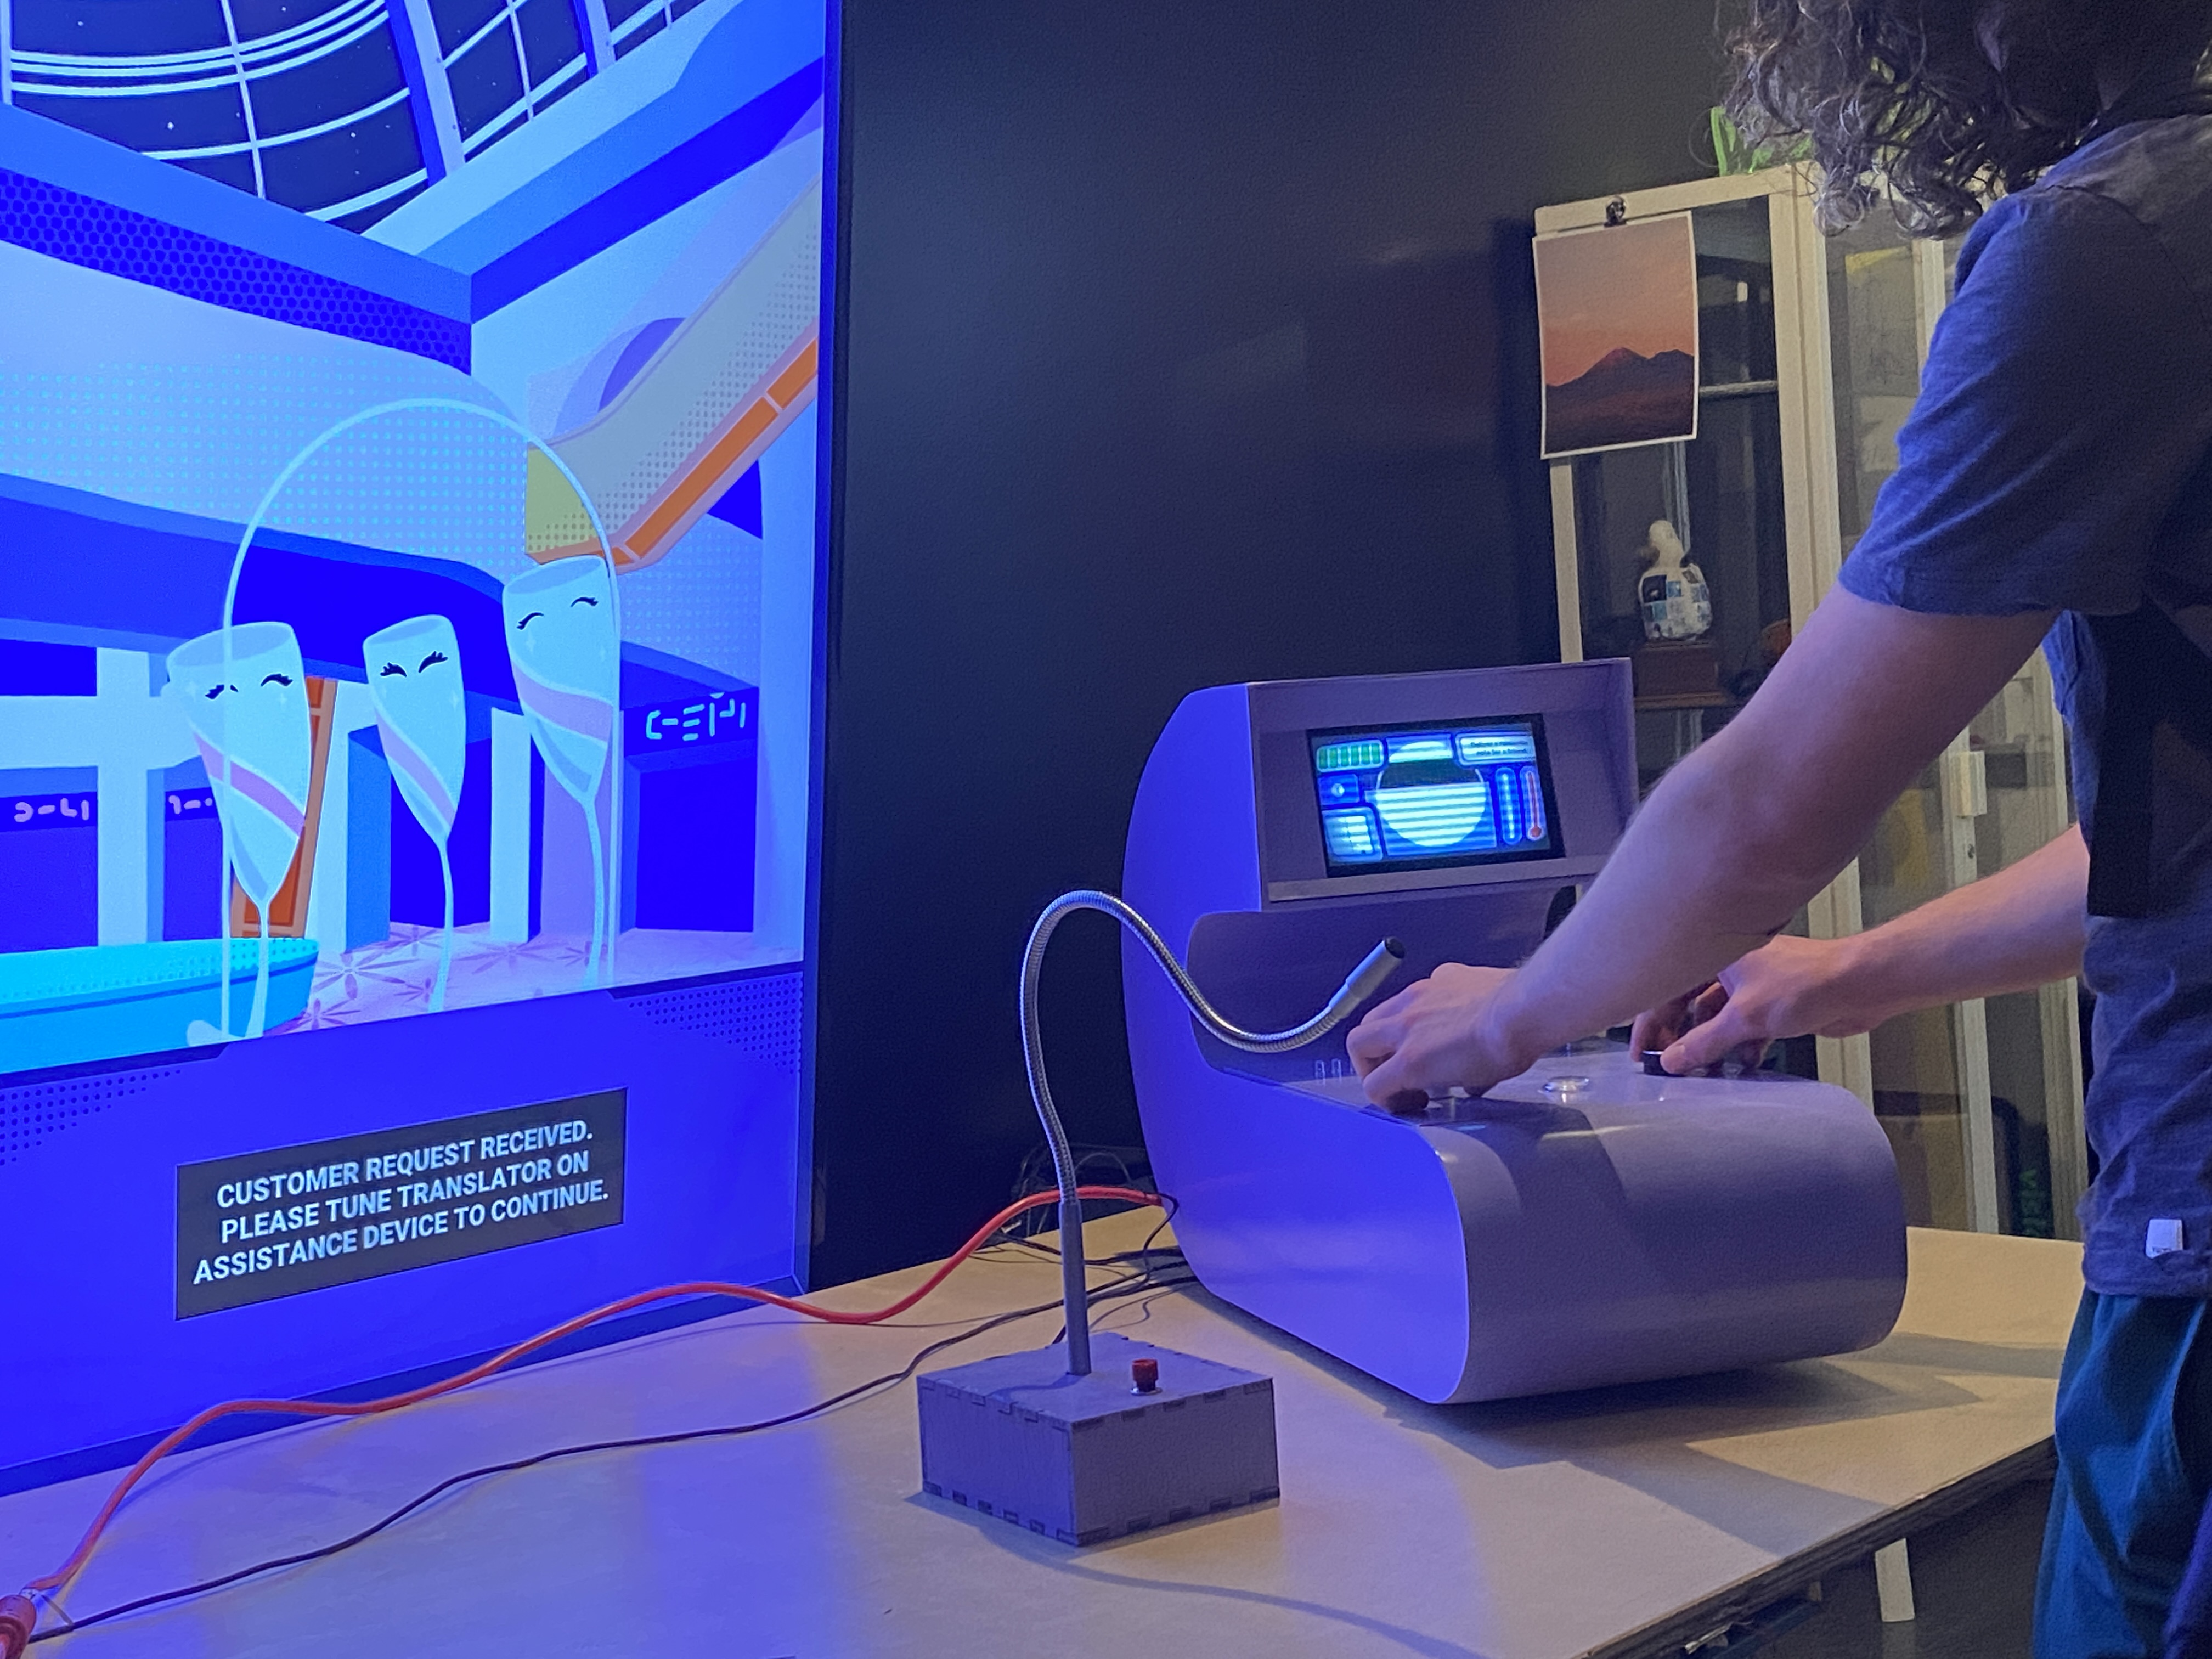
\includegraphics[keepaspectratio,alt={TIKATMOS}]{../Media/tikatmos.jpg}}
\caption{TIKATMOS}
\end{figure}

TIKATMOS is a deeply speculative interactive installation that seeks to
explore gaps in conversation, sustainability, the future of humanity,
and what it means to help using voice-control technology and adaptive
audio. By putting the player in the role of an unidentified species, and
creating a fleshed-out world space, TIKATMOS pokes around some
interesting questions about identity.

\paragraph{Playthings}\label{playthings}

The materiality of the objects in play has a profound effect on the
playful experience. Not only do textures, shapes, and other physical
characteristic communicate essential aspects of these items (which
Fullerton dubs ``resources''), but the very introduction of external
elements themselves communicates something about the playful experience.
A verbal bang, pointed finger, plastic cap-gun, and hyper-realistic 3D
modeled firearm say something of the values at play in the games that
include them, but the presence of weaponry at all as a ``resource''
communicates even more.

The Performative Objects of Kristina Niedderer fit well into this
understanding, as they strategically explore the material and functional
aspects of objects in order to provoke what she calls ``mindful
interactions.'' Their materiality (often at odds with rather than in
service to their functionality) initiates a more reflective stance from
the user within the context of their intended use. Yoko Ono's ``Play it
by Heart'' is another clear example of how the materiality of an object
can be at service for both play and contemplation.

``Performative resources'' seems then to be a fertile space for
exploration (albeit not a great name). Within this understanding, a
designer would create material objects for play in which their
materiality informs both the playful act and the associated
contemplative experience.

\begin{figure}
\centering
\pandocbounded{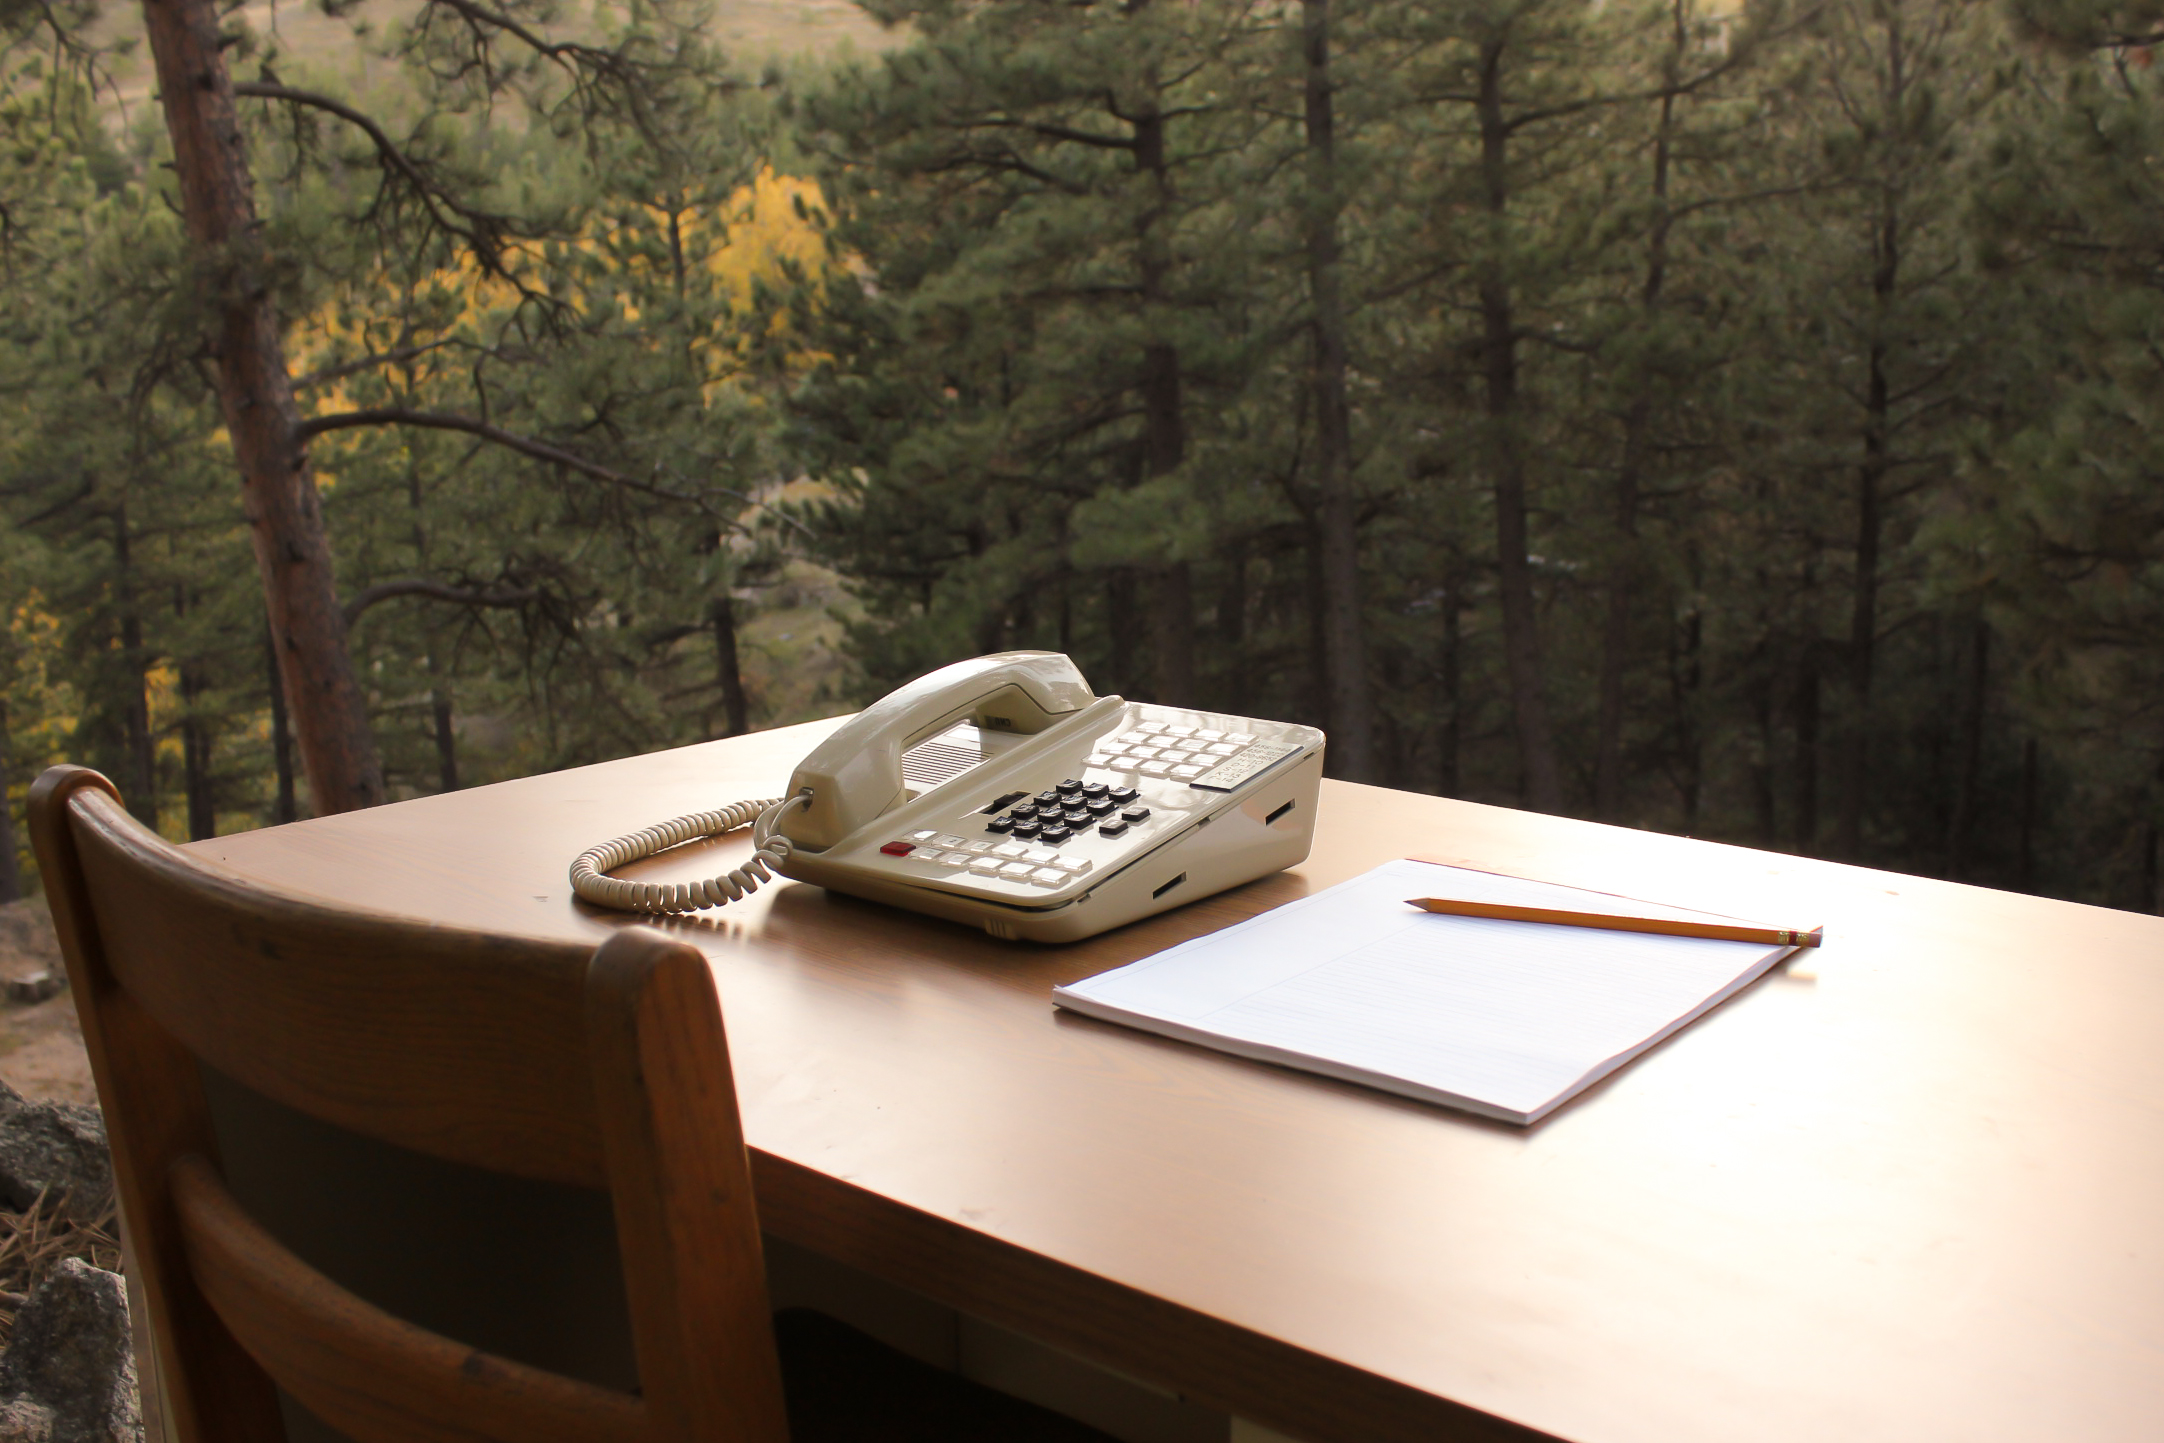
\includegraphics[keepaspectratio,alt={Please Hold}]{../Media/ph.jpg}}
\caption{Please Hold}
\end{figure}

Alt-ctrl is specifically interested in an expansion of the ``stuff'' of
games. We build alt-ctrl installations to ask, ``what if a phone was a
controller,'' or ``what if a series of hold menus could be playful?''
Games like TIKATMOS, Busy Work, Buy Sell, and Please Hold (above) rely
on their objects for the player to interact with. These objects
communicate the game world, but they also can work in cooperation with
(or opposition to) their perceived uses. A phone communicates
``phone-ness'' but does the playful experience hidden within become
stronger by breaking free of its mundane appearance?

\paragraph{Playtime}\label{playtime}

In \emph{Das Spiel. Theorien des Spiels}, Hans Scheuerl argues that
``play is always a `playing between'\,'' various characteristics like
seriousness and pleasure, rules and chance, focused effort and ease.
This concept of `ambivalence,' in conjunction with Csikszentmihalyi's
`flow' helps to explain the playful state. The oscillation between the
states is where play exists. Salen and Zimmerman use the example of the
`play' in a steering wheel.

Ambient Media also relies on this tension between something that can
demand focused attention but also exist entirely in the background. Eno
imagined his ambient music as the soundscape to an environment, ever
present, always playing, with the listener able to tune-in or out as
they pleased. Games like Oreilly's \emph{Mountain} are examples of how
`ambient games' might function, in which the player's attention can
traverse this ambivalent space at will.

How can the concept of ambient ambivalence be leveraged in regards to
time? How can we move the playing of games \emph{away} from flow-focused
and mark the passing of time for contemplative ends? Note: PB's
statement of ``time is one of the most valuable resources that we ask of
our players'' is of particular note here.

\begin{figure}
\centering
\pandocbounded{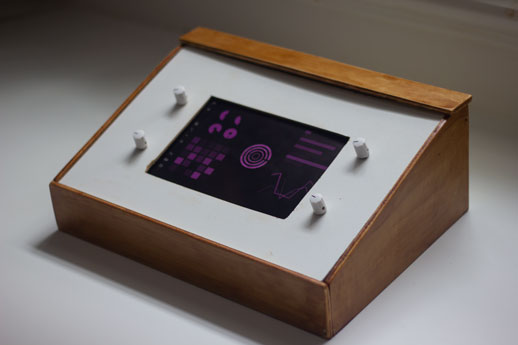
\includegraphics[keepaspectratio,alt={Lest Ten Horizons Cry}]{../Media/lthc.jpg}}
\caption{Lest Ten Horizons Cry}
\end{figure}

\emph{Lest Ten Horizons Cry}~is an exploration in how we can explore
game spaces with traditional electronic instrument interfaces. In this
way, the design of this experience is also deeply concerned with
material object, but ths way that that interaction changes over time is
the most relevant here. Initially, users are presented with a
custom-built boutique synthesizer. By turning the dials, the various
sonic parameters can be adjusted, creating an ever-evolving sonic
landscape. The large synthesizer screen displays simple, cryptic, but
generally traditional visuals mapped to each of these physical dials. It
is only after focused attention from the player that another world can
be discovered. And this attention is not required. Only a player who is
willing to engage with a seemingly ``difficult'' interface is rewarded
with this experience.

\begin{figure}
\centering
\pandocbounded{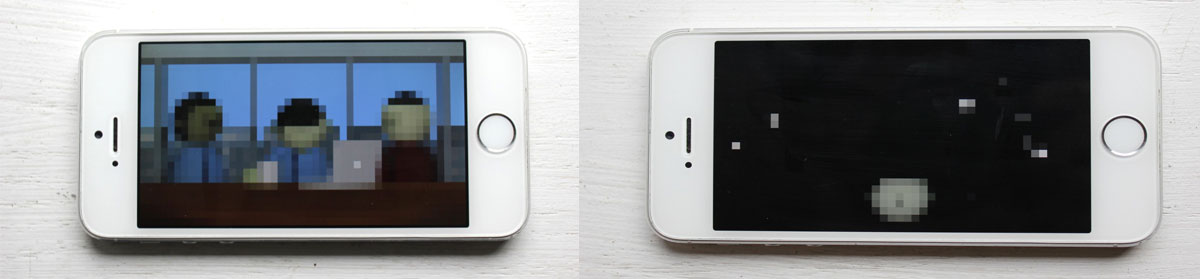
\includegraphics[keepaspectratio,alt={The Meeting}]{../Media/themeeting.jpg}}
\caption{The Meeting}
\end{figure}

The Meeting functions on a similar concept. What looks on the surface
like a standard ``clicker game'' becomes an entirely different
experience if the user refuses to interact with it the way it seems to
communicate that it should be interacted with (i.e to \emph{not} touch
it; to \emph{not} click)

\subsection*{References}\label{references}
\addcontentsline{toc}{subsection}{References}

\protect\phantomsection\label{refs}
\begin{CSLReferences}{1}{1}
\bibitem[\citeproctext]{ref-hanVitaContemplativaPraise2023}
Han, B. C., and D. Steuer. 2023. \emph{Vita {Contemplativa}: {In Praise}
of {Inactivity}}. Polity Press, 2023.
\url{https://books.google.ca/books?id=edzeEAAAQBAJ}.

\end{CSLReferences}

\end{document}
